% =============================================================================
% Chapter 3 — System Description
% Tara Torbati — Master's Thesis
% =============================================================================

\chapter{System Description}
\label{chap:system}

\section{Overview of the Virtual Plant Architecture}
\label{sec:sys-overview}

The empirical evaluation of constrained irrigation controllers requires a
simulation environment that is, simultaneously, physically faithful enough
to expose the agronomic and hydrological consequences of control decisions,
and computationally tractable enough to support both nonlinear optimization
within a receding-horizon loop and policy-gradient training over many
millions of environment steps. This chapter presents such an environment:
a 130-agent agent-based model (ABM) of a topographically heterogeneous
rice field located in Gilan Province, Iran. The model is the shared
test bed on which all four controller architectures introduced in
Chapter~\ref{chap:controllers} (the no-irrigation baseline, the
fixed-schedule heuristic, the Model Predictive Controller, and the
Soft Actor-Critic agent) are evaluated under identical climatic forcings,
budget constraints, and physical dynamics.

The ABM extends the topographical irrigation framework of Lopez-Jimenez
et al.~\cite{Lopezjimenez2024,LopezJimenez2022} with three modifications
required for closed-loop optimal control: explicit two-layer hydrological
decoupling between surface ponding and root-zone moisture, a topological
boundary condition that resolves a degenerate runoff sink, and the
introduction of crop-specific evapotranspiration that couples water stress
directly to biomass accumulation. The system is parameterized for the
Hashemi rice cultivar using FAO Irrigation and Drainage Paper~No.~56
\cite{allen1998}, regional agronomic literature for
Gilan~\cite{jalali2021,sadidi2021}, and the soil-hydraulic
parameterization of Rawls et al.~\cite{rawls1982}.

The remainder of this chapter is organized as follows.
Section~\ref{sec:sys-site} presents the study site, the digital elevation
model, and the directed flow graph that governs lateral water exchange
between agents. Section~\ref{sec:sys-climate} describes the meteorological
data sources, the reference evapotranspiration calculation, and the
selection of three representative climate scenarios.
Section~\ref{sec:sys-params} details the soil and crop parameterization.
Section~\ref{sec:sys-abm} presents the complete state-space dynamics of
the ABM. Section~\ref{sec:sys-control} formalizes the action space, the
seasonal water budget constraint, and the initial conditions that define
the constrained optimal control problem.
Section~\ref{sec:sys-eval} describes the unified software architecture
that ensures fair comparison across controller architectures.
Section~\ref{sec:sys-summary} summarizes the chapter and forward-references
Chapter~\ref{chap:controllers}.

\section{Study Site and Topographic Graph}
\label{sec:sys-site}

\subsection{Field Selection and Digital Elevation Model}
\label{ssec:sys-dem}

The study site is a rectangular agricultural plot in Gilan Province on the
southern Caspian coast of Iran, centered at $38.30^{\circ}$N,
$48.85^{\circ}$E. Gilan is the country's principal rice-producing region;
the cultivar Hashemi grown there accounts for a substantial share of
domestic rice consumption~\cite{surfiran2025,jalali2021}. The province
faces increasing pressure from groundwater depletion, agricultural water
subsidies, and the broader water-scarcity dynamics analyzed in
Chapter~\ref{chap:lit}, making it a meaningful regional test case for
constrained agricultural control.

The terrain is represented by a digital elevation model (DEM) obtained
from the USGS Shuttle Radar Topography Mission (SRTM) one-arcsecond
dataset.\footnote{USGS EarthExplorer,
\url{https://earthexplorer.usgs.gov/}} The DEM was clipped to the field
extent and resampled to a $13 \times 10$ grid, producing $N = 130$ agents
each representing approximately $460$~m$^2$ ($\sim$$21 \times 21$~m).
Raw elevations span $111$~m across the field, with high ground forming
ridges along the northwestern boundary and a shallow valley draining
toward the southeast. This elevation gradient generates substantial
lateral water redistribution through surface runoff, motivating the
adoption of a spatially distributed agent-based representation rather
than a lumped-parameter water balance.

\begin{figure}[h]
\centering
% 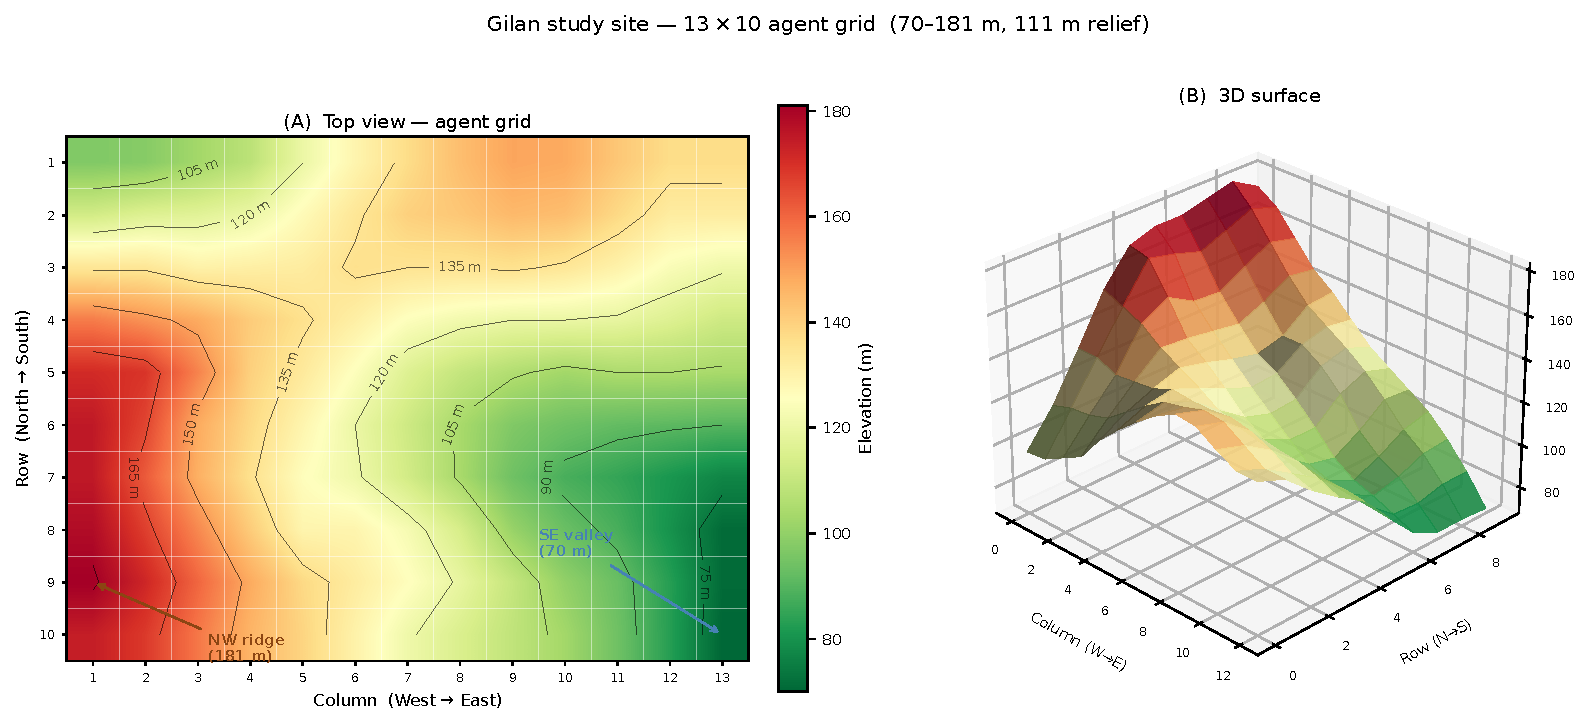
\includegraphics[width=0.85\textwidth]{figures/ch3_dem_heatmap.pdf}
\caption{Digital elevation model of the study site, resampled to the
$13 \times 10$ agent grid. High ground (warm colors) forms ridges in the
northwestern portion of the field; the valley floor (cool colors) drains
toward the southeastern corner.}
\label{fig:dem-heatmap}
\end{figure}

For use within the ABM, raw elevations are normalized to the unit interval
via min--max normalization:
\begin{equation}
\gamma^{(n)} = \frac{z^{(n)} - z_{\min}}{z_{\max} - z_{\min}}, \qquad
\gamma^{(n)} \in [0,1]
\label{eq:elev-norm}
\end{equation}
where $z^{(n)}$ is the raw elevation of agent~$n$. The normalized
elevation $\gamma^{(n)}$ enters the agent state vector as a static
topographic feature and is exposed as an observation to learning-based
controllers.

\subsection{Directed Graph Construction}
\label{ssec:sys-graph}

Lateral surface water exchange is governed by a directed graph
$\mathcal{G} = (\mathcal{V}, \mathcal{E})$ where
$\mathcal{V} = \{1, \ldots, N\}$ indexes the agents and
$\mathcal{E}$ encodes downhill flow directions. Each agent at grid
position $(r, c)$ may exchange water with up to eight neighbors in its
Moore neighborhood. A directed edge $(n, m) \in \mathcal{E}$ is placed
from agent~$n$ to agent~$m$ if and only if
$\gamma^{(m)} < \gamma^{(n)}$, ensuring that water flows strictly
downhill. The number of lower-elevation neighbors of agent~$n$ is
denoted $N_r^{(n)}$ and used in Section~\ref{sec:sys-abm} to allocate
runoff among receivers.

\begin{figure}[h]
\centering
% 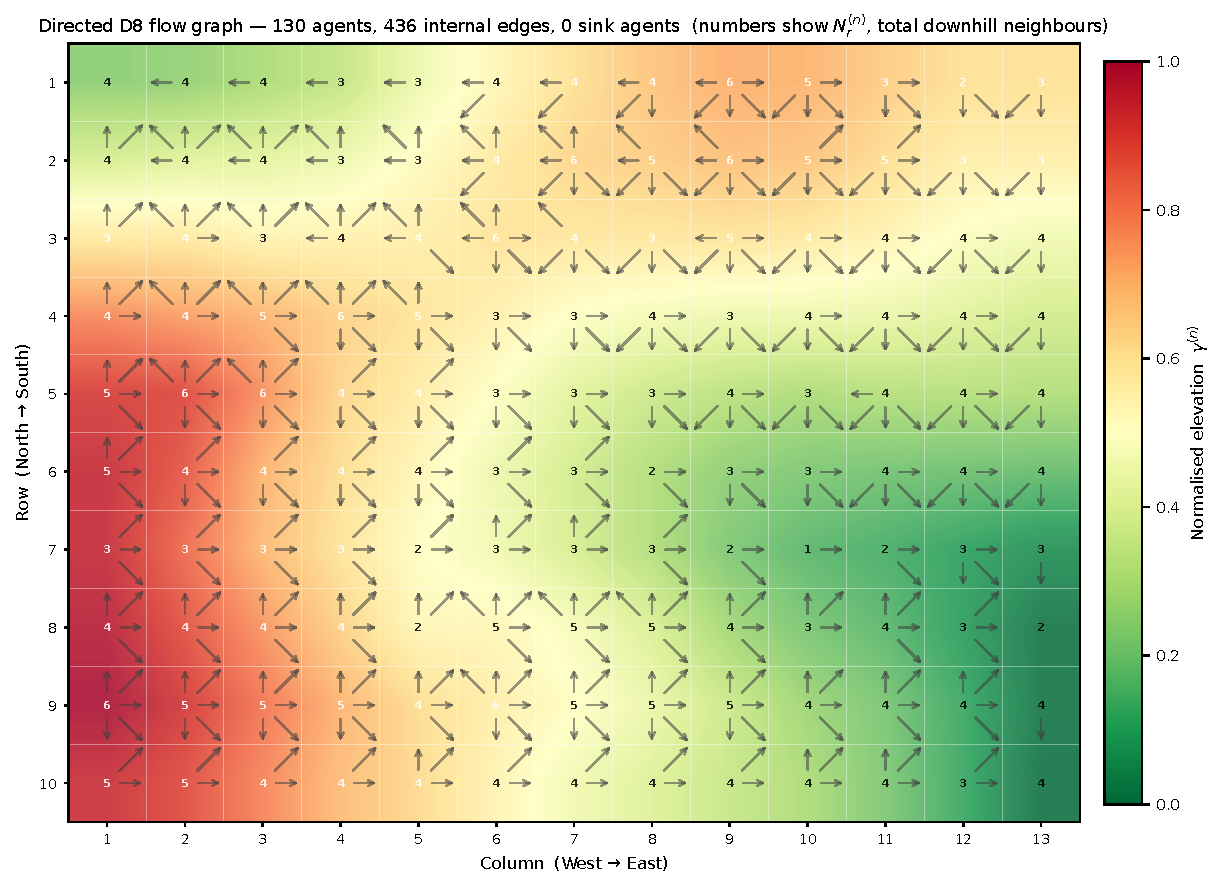
\includegraphics[width=0.85\textwidth]{figures/ch3_flow_graph.pdf}
\caption{Directed flow graph overlaid on the normalized elevation map.
Arrows indicate the direction of lateral surface runoff between agents.
Steep regions exhibit dense, parallel flow lines; the flat valley floor
shows sparser, more diffuse connections.}
\label{fig:flow-graph}
\end{figure}

\subsection{Padded-DEM Boundary Condition}
\label{ssec:sys-padded-dem}

Direct application of the construction above on a finite grid produces a
degenerate boundary condition. Agents at the lowest elevation in the
southeastern corner have no internal lower neighbors and would therefore
satisfy $N_r^{(n)} = 0$. Under the standard runoff routing rule of
\cite{Lopezjimenez2024}, such ``sink'' agents accumulate all incoming
runoff and discharge none, producing unbounded ponding and an artificial
intra-field bathtub effect. The original ABM~\cite{Lopezjimenez2024}
mitigates this by treating sink runoff as physically vanished, but this
violates mass conservation in the surface layer.

To resolve this, the DEM is extended by one cell on each edge through
linear extrapolation of the boundary slopes. Sink-candidate agents
acquire fictitious off-farm lower neighbors in the padded region; these
fictitious cells participate in $N_r^{(n)}$ but are excluded from the
internal state vector. When an agent's runoff is divided among its $N_r$
downhill neighbors, the fraction directed toward off-farm cells is
implicitly removed from the closed system, modeling drainage out of the
field domain. This convention preserves mass conservation across the
internal field while eliminating the bathtub artifact, and is used
throughout this thesis.

\section{Climate Data and Scenarios}
\label{sec:sys-climate}

\subsection{Data Sources}
\label{ssec:sys-data-sources}

Daily meteorological forcings are obtained from the NASA POWER reanalysis
\cite{nasa-power} at the field coordinates ($38.30^{\circ}$N,
$48.85^{\circ}$E), retrieved through the Data Access Viewer single-point
service. The dataset spans the 25-year period 2000--2025 and provides:
mean, maximum, and minimum 2~m air temperature
(\texttt{T2M}, \texttt{T2M\_MAX}, \texttt{T2M\_MIN});
2~m dew point (\texttt{T2MDEW}); corrected daily precipitation
(\texttt{PRECTOTCORR}); 2~m relative humidity (\texttt{RH2M}); surface
shortwave downward irradiance (\texttt{ALLSKY\_SFC\_SW\_DWN}); 2~m wind
speed (\texttt{WS2M}); and surface pressure (\texttt{PS}). The series
were filtered to the agricultural season (April through October), yielding
$5{,}564$ daily records with no missing values. A single anomalous record
(375~mm of rainfall on 7~April 2022) was identified as a likely sensor
artifact and replaced with the calendar-day average of 1.2~mm to prevent
distortion of the seasonal water balance.

\subsection{Reference Evapotranspiration}
\label{ssec:sys-et0}

Reference evapotranspiration $\mathrm{ET}_0$ is the principal driver of
crop water demand in the model. Two standard estimators were evaluated:
the temperature-based Hargreaves formulation and the FAO Penman--Monteith
equation~\cite{allen1998}. The FAO Penman--Monteith equation is
\begin{equation}
\mathrm{ET}_0^{\mathrm{PM}} = \frac{
0.408 \, \Delta (R_n - G) +
\gamma \, \frac{900}{T+273} u_2 (e_s - e_a)
}{
\Delta + \gamma (1 + 0.34 u_2)
}
\label{eq:penman-monteith}
\end{equation}
where $\Delta$ is the slope of the vapor-pressure curve (kPa/$^{\circ}$C),
$R_n$ is the net radiation at the crop surface (MJ/m$^2$/day), $G$ is the
soil heat flux (MJ/m$^2$/day), $\gamma$ is the psychrometric constant
(kPa/$^{\circ}$C), $T$ is the mean 2~m air temperature ($^{\circ}$C),
$u_2$ is the 2~m wind speed (m/s), and $(e_s - e_a)$ is the
saturation-vapor-pressure deficit (kPa).

Across the 25-year rice growing season the Hargreaves and Penman--Monteith
estimators are strongly correlated ($r = 0.94$), but Hargreaves
systematically underestimates evaporative demand by approximately 8.6\%
(seasonal mean $\mathrm{ET}_0 = 4.59$ mm/day vs.\ 5.02 mm/day). The
underestimation arises because Hargreaves uses the diurnal temperature
range $T_{\max} - T_{\min}$ as a proxy for atmospheric demand; in Gilan's
moderated coastal climate, the diurnal range is attenuated
($\Delta T \approx 9.4^{\circ}$C), which biases the estimator downward.
The Penman--Monteith equation, which incorporates radiation, humidity,
and aerodynamic conductance directly, is therefore adopted as the
$\mathrm{ET}_0$ source throughout this thesis.

\subsection{Twenty-Five Year Climatology and Scenario Selection}
\label{ssec:sys-scenarios}

The 25-year climatology exhibits the characteristic features of Gilan's
Caspian climate. Mean daily air temperature ranges from $12^{\circ}$C in
early April to $26^{\circ}$C in mid-July; precipitation shows a dry
mid-season trough (June through August, 0.5--1.5 mm/day) flanked by
wetter shoulder months; solar radiation peaks at $26$ MJ/m$^2$/day in
June; and relative humidity remains in the 60--75\% range throughout.
These conditions create a hot, humid growing environment that is
hydrologically supplied largely by irrigation rather than by in-season
rainfall.

\begin{figure}[h]
\centering
% \includegraphics[width=0.85\textwidth]{figures/ch3_climatology.pdf}
\caption{Twenty-five year daily-average climate at the study coordinates
(2000--2025): rainfall (top), reference evapotranspiration $\mathrm{ET}_0$
(middle), and 2~m air temperature (bottom) over the
April--October agricultural window.}
\label{fig:climatology}
\end{figure}

To evaluate controller performance under varying climatic conditions
without resorting to synthetic weather generation, three years from the
25-year record were selected as representative scenarios:
\begin{itemize}
\item \textbf{Dry scenario (2022):} 39.7~mm of total rice-season rainfall,
near the lower extreme of the climatological distribution. This scenario
stresses the controller's ability to allocate a constrained water budget
under near-zero rainfall augmentation.
\item \textbf{Moderate scenario (2020):} 42.1~mm of rice-season rainfall,
close to the multi-decadal climatological median. This scenario serves
as the baseline operating regime.
\item \textbf{Wet scenario (2024):} 176.8~mm of rice-season rainfall,
substantially above the climatological average. This scenario tests the
controller's ability to capitalize on natural rainfall and to manage
waterlogging risk in low-elevation agents.
\end{itemize}

The three scenarios are summarized in Table~\ref{tab:scenarios}. Selecting
real years from the historical record, rather than synthesizing
statistical extremes, preserves the natural temporal correlation
structure of weather (multi-day rainfall events, heat waves, dry spells)
that synthetic generators tend to attenuate.

\begin{table}[h]
\centering
\caption{Selected climate scenarios for controller evaluation. Total
rainfall is computed over the 93-day rice growing season
(20~May--20~August).}
\label{tab:scenarios}
\begin{tabular}{lcc}
\toprule
\textbf{Scenario} & \textbf{Year} & \textbf{Total rainfall (mm)} \\
\midrule
Dry      & 2022 & 39.7 \\
Moderate & 2020 & 42.1 \\
Wet      & 2024 & 176.8 \\
\bottomrule
\end{tabular}
\end{table}

\section{Soil and Crop Parameterization}
\label{sec:sys-params}

\subsection{Soil Parameters}
\label{ssec:sys-soil}

The soil at the study site is classified as silty loam, consistent with
regional FAO soil maps for the Caspian lowland. Soil hydraulic properties
follow the FAO~Irrigation and Drainage Paper No.~56
recommendations~\cite{allen1998} and the parameter database of
Rawls et al.~\cite{rawls1982} for this textural class. The values used
in the ABM are summarized in Table~\ref{tab:soil-params}.

\begin{table}[h]
\centering
\caption{Soil hydraulic parameters for silty loam.}
\label{tab:soil-params}
\begin{tabular}{lccl}
\toprule
\textbf{Parameter} & \textbf{Symbol} & \textbf{Value} & \textbf{Source} \\
\midrule
Water uptake coefficient            & $\theta_1$    & 0.096  & \cite{Lopezjimenez2024} \\
Wilting point (vol.\ fraction)      & $\theta_2$    & 0.15   & \cite{allen1998} \\
SCS curve-number threshold (mm)     & $\theta_3$    & 10.0   & \cite{Lopezjimenez2024} \\
Daily drainage coefficient          & $\theta_4$    & 0.05   & \cite{Lopezjimenez2024} \\
Field capacity (vol.\ fraction)     & $\theta_6$    & 0.35   & \cite{allen1998} \\
Saturation (vol.\ fraction)         & $\theta_{\mathrm{sat}}$ & 0.50 & \cite{rawls1982} \\
\bottomrule
\end{tabular}
\end{table}

These parameters define the principal hydrological reference levels used
by the ABM and the controllers: the wilting point
$\mathrm{WP} = \theta_2 \theta_5 = 60$~mm, the field capacity
$\mathrm{FC} = \theta_6 \theta_5 = 140$~mm, and the saturation level
$\theta_{\mathrm{sat}} \theta_5 = 200$~mm, where $\theta_5$ is the
crop-specific root-zone depth.

\subsection{Hashemi Rice Cultivar}
\label{ssec:sys-rice}

Hashemi is the dominant rice cultivar grown in Gilan and is the crop
modeled in this thesis. Phenological and physiological parameters
follow standard agronomic conventions and are calibrated where necessary
against regional measurements.

The base temperature for thermal-time accumulation is set to
$\theta_7 = 10^{\circ}$C, following standard Growing-Degree-Day (GDD)
conventions for cereal crops~\cite{mcmaster1997,laohasiriwong2023} and
consistent with the baseline ABM~\cite{Lopezjimenez2024}. The maturity
threshold is calibrated to $\theta_{18} = 1{,}250\,^{\circ}\mathrm{C}\cdot$day
based on the 25-year temperature record and validated against local
field measurements that report 1{,}216--1{,}352~GDD for Hashemi in
Gilan~\cite{sadidi2021}. The crop coefficient is
$K_c = 1.15$~\cite{allen1998,jalali2021}, the root-zone depth is
$\theta_5 = 400$~mm, and the drought sensitivity is $\theta_{14} = 0.80$,
reflecting rice's known intolerance to soil-moisture deficits.

Transplanting is simulated on 20~May (DOY~141), aligning with local
practice when the seven-day rolling-average mean temperature reaches
$18^{\circ}$C and the minimum temperature reaches
$12^{\circ}$C~\cite{faghani2011,sarma2018}. Harvest occurs on
20~August (DOY~233), yielding a 93-day field season. Extending the
season beyond this date sharply increases exposure to extreme rainfall
events ($\geq$~20~mm/day under WMO R20mm criteria) that cause crop
lodging~\cite{nayak2011,raoufi2025,tasteiran_harvest}.

The 20-day prior nursery period contributes initial conditions
$x_2(0) = 210\,^{\circ}\mathrm{C}\cdot$day for thermal time and
$x_4(0) = 60$~g/m$^2$ for biomass at field transplanting.

\subsection{Parameter Summary}
\label{ssec:sys-paramsum}

Table~\ref{tab:crop-params} summarizes the crop-specific parameters used
throughout the thesis. The harvest index $\mathrm{HI} = 0.42$ is used
to convert simulated dry biomass at harvest ($x_4$, g/m$^2$) to
agronomic yield via $Y = x_4 \cdot \mathrm{HI} \cdot 10$ (kg/ha).

\begin{table}[h]
\centering
\caption{Crop-specific ABM parameters for Hashemi rice.}
\label{tab:crop-params}
\begin{tabular}{llcl}
\toprule
\textbf{Parameter} & \textbf{Symbol} & \textbf{Value} & \textbf{Source} \\
\midrule
Root-zone depth                       & $\theta_5$         & 400~mm                         & \cite{allen1998} \\
Base temperature                      & $\theta_7$         & $10^{\circ}$C                  & \cite{mcmaster1997} \\
Heat-stress onset                     & $\theta_9$         & $35^{\circ}$C                  & \cite{allen1998} \\
Extreme heat                          & $\theta_{10}$      & $42^{\circ}$C                  & \cite{laohasiriwong2023} \\
Heat-stress maturation rate           & $\theta_{11}$      & 0.0030                         & \cite{Lopezjimenez2024} \\
Drought-stress maturation rate        & $\theta_{12}$      & 0.0030                         & \cite{Lopezjimenez2024} \\
Radiation use efficiency              & $\theta_{13}$      & 0.65                           & \cite{patel2013,sadras2021} \\
Drought sensitivity                   & $\theta_{14}$      & 0.80                           & \cite{Lopezjimenez2024} \\
Maturity threshold (GDD)              & $\theta_{18}$      & 1{,}250                        & \cite{sadidi2021} \\
Maximum interception                  & $\theta_{19}$      & 0.95                           & \cite{Lopezjimenez2024} \\
GDD at 50\% interception              & $\theta_{20}$      & 417                            & \cite{paredes2025} \\
Crop coefficient                      & $K_c$              & 1.15                           & \cite{allen1998,jalali2021} \\
Depletion fraction                    & $p$                & 0.20                           & \cite{allen1998} \\
Harvest index                         & $\mathrm{HI}$      & 0.42                           & \cite{jalali2021} \\
Initial thermal time (transplanting)  & $x_2(0)$           & 210~$^{\circ}\mathrm{C}\cdot$day  & calibrated \\
Initial biomass (transplanting)       & $x_4(0)$           & 60~g/m$^2$                     & estimated \\
\bottomrule
\end{tabular}
\end{table}

All parameters in Tables~\ref{tab:soil-params} and \ref{tab:crop-params}
are drawn from peer-reviewed agronomic literature, the FAO Irrigation
and Drainage Paper No.~56~\cite{allen1998}, or are calibrated against
regional Hashemi rice measurements~\cite{sadidi2021,jalali2021}.
Empirical validation of the integrated ABM dynamics against field
observations in Gilan is outside the scope of this thesis and is
identified as a direction for future work.

\section{Agent-Based Model Equations}
\label{sec:sys-abm}

The crop-soil system is represented as $N = 130$ coupled discrete-time
dynamical systems. At each daily timestep $k \in \{0, \ldots, K-1\}$
with $K = 93$, agent $n \in \{1, \ldots, N\}$ maintains the state
vector
\begin{equation}
\mathbf{x}^{(n)}(k) = \begin{bmatrix}
x_1^{(n)}(k) \\
x_2^{(n)}(k) \\
x_3^{(n)}(k) \\
x_4^{(n)}(k) \\
x_5^{(n)}(k)
\end{bmatrix}
=
\begin{bmatrix}
\text{root-zone soil water (mm)}\\
\text{cumulative thermal time (}^{\circ}\mathrm{C}\cdot\text{day)}\\
\text{cumulative maturation (---)} \\
\text{aboveground dry biomass (g/m}^2\text{)} \\
\text{surface ponding depth (mm)}
\end{bmatrix}
\label{eq:state-vec}
\end{equation}
The control input $u^{(n)}(k) \in [0, u_{\max}]$ is the daily irrigation
volume (mm) applied to agent~$n$. To accurately simulate lateral water
redistribution while maintaining computational efficiency, the field is
solved sequentially within each timestep following a topological sort
of the directed flow graph: agents are processed from highest to
lowest elevation, ensuring that all uphill contributions to a given
agent are already computed by the time that agent is updated.
Subsurface lateral flow is omitted on the basis that, at the
$\sim$$460$~m$^2$ agent resolution and over the daily timestep, lateral
movement through silty loam is small compared to vertical drainage and
overland flow; agents are coupled exclusively through the surface
runoff graph.

The remainder of this section presents the components of the daily
state-update map
$\mathbf{x}^{(n)}(k+1) = f(\mathbf{x}^{(n)}(k), u^{(n)}(k), \mathbf{w}(k); \mathcal{G})$,
where $\mathbf{w}(k)$ collects the daily climate forcings.

\subsection{Surface Hydrology and Topographic Cascade Routing}
\label{ssec:sys-surface}

The total surface water available to agent $n$ at timestep $k$
aggregates yesterday's un-infiltrated ponding, daily precipitation,
applied irrigation, and routed runoff from all uphill neighbors:
\begin{equation}
W_{\mathrm{surf}}^{(n)}(k) = x_5^{(n)}(k) + P(k) + u^{(n)}(k)
+ \sum_{m \in U(n)} \frac{\phi_2^{(m)}(k)}{N_r^{(m)}}
\label{eq:wsurf}
\end{equation}
where $P(k)$ is the daily rainfall, $U(n)$ is the set of uphill
neighbors of agent~$n$, $\phi_2^{(m)}(k)$ is the runoff generated by
neighbor~$m$, and $N_r^{(m)}$ is the total number of downhill
neighbors of~$m$ (including off-farm neighbors arising from the
padded-DEM convention of Section~\ref{ssec:sys-padded-dem}). The
division by $N_r^{(m)}$ allocates outgoing runoff equally among
receivers; the fraction directed to off-farm cells is implicitly
removed from the closed system.

Surface runoff $\phi_2^{(n)}(k)$ is computed using the SCS curve-number
formulation with threshold $\theta_3$:
\begin{equation}
\phi_2^{(n)}(k) =
\begin{cases}
\dfrac{\bigl(W_{\mathrm{surf}}^{(n)}(k) - \theta_3\bigr)^2}
      {W_{\mathrm{surf}}^{(n)}(k) + 4\theta_3},
& \text{if } N_r^{(n)} > 0 \text{ and } W_{\mathrm{surf}}^{(n)}(k) > \theta_3 \\
0, & \text{otherwise}
\end{cases}
\label{eq:phi2}
\end{equation}
The boundary condition $\phi_2^{(n)} = 0$ for sink-candidate agents
($N_r^{(n)} = 0$ in the unpadded sense) is preserved here for
robustness; under the padded-DEM convention these cases do not occur
in practice because all internal agents acquire at least one external
downhill neighbor.

\subsection{Subsurface Hydrology and Infiltration}
\label{ssec:sys-subsurface}

Crop-specific evapotranspiration $\mathrm{ET}_c$ scales the reference
evapotranspiration by the crop coefficient:
\begin{equation}
\mathrm{ET}_c(k) = K_c \cdot \mathrm{ET}_0(k)
\label{eq:etc}
\end{equation}
Crop transpiration $\phi_1^{(n)}$ is the volume actually withdrawn by
plant roots, bounded above by atmospheric demand and below by the
available extractable water:
\begin{equation}
\phi_1^{(n)}(k) = \min\Bigl(
\max\bigl(\theta_1 (x_1^{(n)}(k) - \theta_2 \theta_5),\, 0\bigr),
\, \mathrm{ET}_c(k)
\Bigr)
\label{eq:phi1}
\end{equation}
Water that does not run off the surface infiltrates the root zone.
Infiltration is bounded by the soil's saturation capacity to prevent
nonphysical pooling within the root zone:
\begin{align}
I_{\max}^{(n)}(k) &= \theta_{\mathrm{sat}} \theta_5
- x_1^{(n)}(k) + \phi_1^{(n)}(k)
\label{eq:imax}\\
I^{(n)}(k) &= \min\bigl(
W_{\mathrm{surf}}^{(n)}(k) - \phi_2^{(n)}(k),\,
I_{\max}^{(n)}(k)
\bigr)
\label{eq:i}
\end{align}
A temporary intra-day moisture state is computed before drainage:
\begin{equation}
x_{1,\mathrm{temp}}^{(n)}(k) = x_1^{(n)}(k) + I^{(n)}(k) - \phi_1^{(n)}(k)
\label{eq:x1temp}
\end{equation}
If this exceeds field capacity, a fraction of the excess drains
vertically to deep percolation:
\begin{align}
E_{\mathrm{sub}}^{(n)}(k) &= \max\bigl(
x_{1,\mathrm{temp}}^{(n)}(k) - \theta_6 \theta_5,\, 0
\bigr)
\label{eq:esub}\\
\phi_3^{(n)}(k) &= \theta_4 \cdot E_{\mathrm{sub}}^{(n)}(k)
\label{eq:phi3}
\end{align}
The drainage coefficient $\theta_4 = 0.05$ corresponds to a daily
drainage rate of 5\%, so excess water above field capacity persists
for approximately two weeks before fully draining --- a physically
realistic timescale for silty loam.

\subsection{Stress Penalties and Crop Growth}
\label{ssec:sys-stress}

Phenological development is driven by thermal time accumulation:
\begin{equation}
h_1^{(n)}(k) = \max\bigl(T_{\mathrm{mean}}(k) - \theta_7,\, 0\bigr)
\label{eq:h1}
\end{equation}
Heat stress reduces maturation efficiency, and low-temperature stress
prevents biomass accumulation entirely:
\begin{align}
h_2(k) &= \mathrm{clip}\!\left(
\frac{\theta_{10} - T_{\max}(k)}{\theta_{10} - \theta_9},\, 0,\, 1
\right)
\label{eq:h2}\\
h_7(k) &=
\begin{cases}
1, & T_{\mathrm{mean}}(k) > \theta_7 \\
0, & T_{\mathrm{mean}}(k) \leq \theta_7
\end{cases}
\label{eq:h7}
\end{align}
Hydrological stresses act multiplicatively on biomass accumulation.
Drought stress penalizes the system when actual transpiration falls
short of atmospheric demand, while waterlogging stress penalizes
root-zone oxygen deprivation when soil moisture exceeds field
capacity:
\begin{align}
h_3^{(n)}(k) &= 1 - \theta_{14} \cdot
\max\!\left(1 - \frac{\phi_1^{(n)}(k)}{\mathrm{ET}_c(k)},\, 0\right)
\label{eq:h3}\\
h_6^{(n)}(k) &= \mathrm{clip}\!\left(
1 - \frac{x_1^{(n)}(k) - \theta_6 \theta_5}{\theta_6 \theta_5},\,
0,\, 1
\right)
\label{eq:h6}
\end{align}
Note that $h_3$ acts directly on biomass accumulation through
\eqref{eq:x4-update} below. This is a deliberate departure from the
baseline ABM~\cite{Lopezjimenez2024}, in which the drought stress
function influences only the maturation state $x_3$ and thus reduces
biomass only indirectly through advanced senescence. Under the
baseline formulation, an unirrigated rice crop accumulates nearly the
same daily biomass as a fully irrigated crop until late-season
senescence intervenes, which renders the irrigation-vs.-yield
relationship insensitive and obscures the agronomic consequences of
control decisions. Multiplying the radiation-use-efficiency term in
the biomass equation by $h_3$ follows the FAO~AquaCrop
convention~\cite{allen1998} and ensures that drought directly reduces
the daily biomass increment.

The growth function $g(x_2)$ describes the fraction of intercepted
solar radiation contributing to biomass through a two-branch sigmoid
scaled by the maximum interception parameter $\theta_{19}$:
\begin{equation}
g\bigl(x_2^{(n)}\bigr) =
\begin{cases}
\dfrac{\theta_{19}}{1 + \exp\!\bigl(-0.01(x_2^{(n)} - \theta_{20})\bigr)},
& x_2^{(n)} \leq \theta_{18}/2 \\[1.0em]
\dfrac{\theta_{19}}{1 + \exp\!\bigl( 0.01(x_2^{(n)} + x_3^{(n)} - \theta_{18})\bigr)},
& x_2^{(n)} > \theta_{18}/2
\end{cases}
\label{eq:g}
\end{equation}
The first branch represents the rising canopy expansion phase before
mid-season; the second represents post-maturation senescence, in which
the maturation index $x_3$ accelerates the decline of canopy
interception.

\subsection{Complete State-Update Equations}
\label{ssec:sys-update}

Combining the surface, subsurface, and growth components, the daily
state update for agent~$n$ is:
\begin{align}
x_1^{(n)}(k+1) &= x_{1,\mathrm{temp}}^{(n)}(k) - \phi_3^{(n)}(k) \label{eq:x1-update}\\
x_2^{(n)}(k+1) &= x_2^{(n)}(k) + h_1^{(n)}(k) \label{eq:x2-update}\\
x_3^{(n)}(k+1) &= x_3^{(n)}(k) + \theta_{11}\bigl(1 - h_2(k)\bigr)
                                   + \theta_{12}\bigl(1 - h_3^{(n)}(k)\bigr) \label{eq:x3-update}\\
x_4^{(n)}(k+1) &= x_4^{(n)}(k) + \theta_{13} \cdot h_3^{(n)}(k) \cdot
                                   h_6^{(n)}(k) \cdot h_7(k) \cdot
                                   g\bigl(x_2^{(n)}(k)\bigr) \cdot R_s(k) \label{eq:x4-update}\\
x_5^{(n)}(k+1) &= W_{\mathrm{surf}}^{(n)}(k) - \phi_2^{(n)}(k) - I^{(n)}(k) \label{eq:x5-update}
\end{align}
where $R_s(k)$ is the daily incoming shortwave radiation. The biomass
update~\eqref{eq:x4-update} is the central agronomic equation: the
multiplicative coupling of $h_3$, $h_6$, and $h_7$ ensures that any
of drought, waterlogging, or cold stress can independently arrest
growth, while phenological progression $g(x_2)$ scales the
photosynthetic capacity of the canopy. The surface ponding update
\eqref{eq:x5-update} explicitly conserves any water that arrived at
the agent but neither ran off nor infiltrated, preserving it as a
boundary state for the subsequent day --- the mechanism by which
multi-day waterlogging events emerge in low-elevation agents during
prolonged wet periods.

\section{Action Space, Constraints, and Water Budget}
\label{sec:sys-control}

The ABM defined in Section~\ref{sec:sys-abm} provides the dynamics of
the constrained finite-horizon optimal control problem solved by the
controllers in Chapter~\ref{chap:controllers}. This section formalizes
the action space and the global water-budget constraint.

\subsection{Action Space and Actuator Constraints}
\label{ssec:sys-action}

The control action at timestep $k$ is the joint irrigation vector
$\mathbf{u}(k) = [u^{(1)}(k), \ldots, u^{(N)}(k)]^{\top} \in \mathbb{R}^{N}$,
specifying the volume (mm) applied to each of the $N = 130$ agents.
Each per-agent action is bounded by the physical actuator capacity
\begin{equation}
0 \leq u^{(n)}(k) \leq u_{\max}, \qquad u_{\max} = 12 \text{ mm/day}
\label{eq:action-bound}
\end{equation}
The lower bound reflects the irreversibility of the actuator: water can
only be added to the field, never withdrawn. The upper bound corresponds
to the practical capacity of low-pressure surface and drip-line
distribution systems applied over a 24-hour cycle and is consistent with
the maximum daily volume reported in Hashemi rice
practice~\cite{jalali2021}.

\subsection{Seasonal Water Budget}
\label{ssec:sys-budget}

A defining feature of the constrained agricultural control problem is
the existence of a hard, global, season-cumulative water budget. Unlike
infinitely-supplied irrigation systems, real agricultural producers in
water-scarce regions operate under volumetric allocations established
ex~ante by water resource authorities, by deficit-mitigation policy, or
by physical aquifer constraints~\cite{Mesgaran2018,Nouri2023}. The
controller must therefore allocate a finite total volume optimally
across the entire season. This is encoded as the linear constraint
\begin{equation}
\sum_{k=0}^{K-1} \sum_{n=1}^{N} u^{(n)}(k) \leq W_{\mathrm{total}}
\label{eq:budget}
\end{equation}
where $W_{\mathrm{total}}$ is the seasonal allocation in mm field-mean
equivalents. The allocation at full deficit-free supply is computed
from the climatological water balance:
\begin{equation}
W_{\mathrm{total}}^{\mathrm{full}} =
\max\bigl(\mathrm{ET}_c^{\mathrm{seasonal}} -
\bar{P}^{\mathrm{seasonal}},\, 0\bigr)
\label{eq:Wfull}
\end{equation}
where $\mathrm{ET}_c^{\mathrm{seasonal}}$ is the seasonal crop demand
computed from the 25-year climatological mean
$\overline{\mathrm{ET}}_0 \cdot K_c \cdot K$, and
$\bar{P}^{\mathrm{seasonal}}$ is the 25-year average rice-season
rainfall (53.3~mm). For Hashemi rice this evaluates to
$W_{\mathrm{total}}^{\mathrm{full}} = 484$~mm, which agrees closely
with field measurements ranging from 534~mm under
System-of-Rice-Intensification management to 632~mm under
traditional flooding~\cite{jalali2021}.

To evaluate controller robustness under scarcity, two deficit
allocations are also considered:
\begin{itemize}
\item $W_{\mathrm{total}}^{85\%} = 411$~mm (15\% reduction)
\item $W_{\mathrm{total}}^{70\%} = 339$~mm (30\% reduction)
\end{itemize}
These three allocations span the realistic range of deficit-irrigation
prescriptions issued by Iranian water resource
authorities~\cite{Mesgaran2018,Nouri2023} and constitute one of the
two principal axes (alongside climate scenario) of the experimental
grid in Chapter~\ref{chap:results}.

\subsection{Initial Conditions and Episode Structure}
\label{ssec:sys-init}

The agricultural season is initialized at field transplanting
($k = 0$, DOY~141, 20~May) with the following per-agent state:
\begin{equation}
\mathbf{x}^{(n)}(0) = \begin{bmatrix}
140 \text{ mm} \\
210\, ^{\circ}\mathrm{C} \cdot \text{day} \\
0 \\
60 \text{ g/m}^2 \\
0 \text{ mm}
\end{bmatrix}
\label{eq:initial-state}
\end{equation}
The initial soil moisture $x_1(0) = 140$~mm corresponds to field
capacity, reflecting standard transplanting practice in which paddies
are flooded immediately prior to the introduction of seedlings. The
initial thermal time $x_2(0) = 210$~GDD and biomass
$x_4(0) = 60$~g/m$^2$ represent the cumulative state at the end of the
20-day nursery period, calibrated against regional Hashemi development
data~\cite{sadidi2021}. The remaining initial states reflect a dry
field surface with no prior maturation accumulation.

The episode terminates at $k = K = 93$ (DOY~233, 20~August),
corresponding to harvest. Agronomic yield is computed from the final
field-mean biomass via
\begin{equation}
Y = \mathrm{HI} \cdot 10 \cdot \frac{1}{N} \sum_{n=1}^{N} x_4^{(n)}(K)
\quad \text{(kg/ha)}
\label{eq:yield}
\end{equation}
This yield, together with the cumulative water consumption, the
trajectories of $x_1$ and $x_5$, and per-agent stress indicators,
constitutes the principal performance metrics evaluated in
Chapter~\ref{chap:results}.

\section{Unified Software Evaluation Framework}
\label{sec:sys-eval}

To ensure that comparative results across the four controller
architectures evaluated in this thesis are attributable to differences
in control policy rather than to implementation artifacts, the
simulation pipeline is structured into three strictly separated
software layers. This separation, formalized below, eliminates several
common sources of evaluation bias in comparative control studies.

\paragraph{Environment layer.}
The environment layer maintains the true physical state
$\mathbf{X}(k) \in \mathbb{R}^{5 \times N}$ of the field, executes the
topographic cascade routing using the high-fidelity ABM defined in
Section~\ref{sec:sys-abm}, and computes the deterministic state
transition $\mathbf{X}(k+1) = f(\mathbf{X}(k), \mathbf{U}(k), \mathbf{w}(k))$.
This layer is identical for all controllers and is never modified or
approximated during evaluation. In particular, controllers that rely
on a control-oriented surrogate model (such as the MPC of
Chapter~\ref{chap:controllers}) operate on the surrogate internally
but are evaluated on the unmodified ABM.

\paragraph{Controller layer.}
The controller layer provides a standardized interface. All controllers
inherit from a common abstract base class and must implement a single
method,
\[
\texttt{get\_action(state, forecast)} \to \mathbf{u}(k) \in \mathbb{R}^N,
\]
that maps the current physical state and an optional weather forecast
to a joint action. This guarantees that the heavyweight nonlinear
program solver of MPC and the trivial zero-action of the no-irrigation
baseline interact with the environment through identical APIs, and
that no controller can use information not also available to the
others.

\paragraph{Runner layer.}
The runner layer is a centralized orchestrator that drives the
day-by-day simulation. At each timestep $k$, it (i) queries the
controller for an action $\mathbf{u}(k)$, (ii) clips the action to
satisfy the per-agent bounds and the remaining seasonal budget,
(iii) applies the action to the environment, (iv) advances the
environment by one day, (v) deducts the applied volume from the
budget counter, and (vi) logs the complete state, action, climate
forcing, and diagnostic information to a long-format Parquet file with
a JSON metadata sidecar. The post-action budget clipping is identical
across controllers: a controller cannot circumvent
\eqref{eq:budget} regardless of its internal policy.

This three-layer architecture guarantees that any difference in
agronomic outcome (yield, water consumption, stress-day count) between
two controllers is strictly attributable to the policies themselves,
not to differences in physical simulation, budget enforcement, or
logging granularity.

\section{Chapter Summary}
\label{sec:sys-summary}

This chapter has presented the constrained virtual plant on which the
controller comparisons in Chapters~\ref{chap:controllers} and
\ref{chap:results} are conducted. The plant is a 130-agent ABM of a
topographically heterogeneous Hashemi rice field in Gilan Province,
Iran, parameterized from FAO Irrigation and Drainage Paper No.~56
\cite{allen1998}, regional agronomic measurements
\cite{jalali2021,sadidi2021}, and the soil-hydraulic database of Rawls
et al.~\cite{rawls1982}. The ABM extends the topographical framework
of Lopez-Jimenez et al.~\cite{Lopezjimenez2024} with three
modifications required for closed-loop control: explicit decoupling
between surface ponding and root-zone moisture, a padded-DEM boundary
condition that resolves a degenerate sink behavior in the original
formulation, and crop-specific evapotranspiration with drought stress
acting directly on biomass accumulation.

The constrained optimal control problem has been formalized: the daily
control action is a 130-dimensional irrigation vector bounded above by
the physical actuator capacity, subject to a seasonal water-budget
constraint of 484~mm at full allocation, with deficit scenarios at
85\% and 70\% allocation evaluated for robustness. Three climate
scenarios drawn from the 25-year NASA POWER record (dry 2022,
moderate 2020, wet 2024) span the relevant range of seasonal rainfall
conditions for the study site. A unified three-layer software
evaluation framework guarantees implementation-bias-free comparison
across controllers.

The next chapter introduces the four controller architectures
evaluated on this plant: the no-irrigation baseline that establishes
the rainfed yield floor, the fixed-schedule heuristic representing
traditional Gilan irrigation practice, the constrained Model
Predictive Controller, and the Soft Actor-Critic reinforcement
learning agent. The cost-function design, the symbolic-graph
implementation of the predictive controller, and the
centralized-training-decentralized-execution architecture of the
learning agent are presented in turn, together with the weight
sensitivity analysis that calibrates the cost-function trade-offs to
real Iranian water-pricing tiers.
